\chapter{Case Studies in English Diachrony}\label{ch:diachron}
\section{Introduction}
This chapter supports the claims made in the previous three chapters with three case studies in the development of recipient ditransitive syntax in the history of English. The first case study examines changes in the realisation of the dative P head. The second case study examines recipient passivisation. The third deals with the rate of passivisation from underlyingly RT (recipient--theme) word orders. As discussed in the introduction, quantitative (and especially) diachronic studies can provide a useful independent verification of analyses developed on the basis of acceptability judgements. Crucially, data from systematic patterns in language production can provide independent verification of theories developed primarily from language comprehension (i.e., acceptability judgements). This chapter begins with an introduction to the quantitative study of historical syntax, focussing primarily on statistical methods of extracting information from quantitative data. This background section is followed by a discussion of each of the case studies mentioned above. The conclusion summarises the case study results and considers broader implications for work on diachronic syntax.

\section{Quantitative Study of Historical Syntax}\label{sec:log-reg}
	Under the (commonly adopted) Borer--Chomsky Conjecture \citep{Baker.2008}, syntactic variation is driven by features of functional lexical items. Under this system, the syntactic machinery is universal and differences in the lexicon of functional items are the only points of syntactic variation. The presence/absence of a syntactic operation is formally implemented as the presence/absence of a particular feature on a functional head. Thus, syntactic change involves the addition, removal or replacement of functional items in the lexicon.

	Morphological change (especially with respect to allomorphy) can be thought of in similar terms. This analogy can be seen in the Distributed Morphology (DM) formalism \citep{Halle.1993}. In DM, allomorphy is captured by the use of vocabulary items, which formalise the relationship between syntactic/semantic features and phonological forms. Each vocabulary item must contain a set of syntactic/semantic features and a phonological form (e.g., /z/ $\leftrightarrow$ [+pl] for English plurals). A vocabulary item can also contain a context in which the item applies (e.g., /n/ $\leftrightarrow$ [+pl] / [OX,\dots]$^{\smallfrown}$\_ captures the allomorphy in plural suffixes producing English \textit{oxen}). The Subset Principle of DM (related to Panini's Elsewhere Principle) states that when multiple vocabulary items could apply (for example the contextual conditions of both the regular /z/ and irregular /n/ forms are met with the root OX), the more specific item is used (in this case the irregular /n/ form). Changes in allomorphy, thus, reflect the addition, removal or replacement of vocabulary items.

	Both syntactic and morphological changes have two stages. In order for the change to begin, some language user needs to innovate a new form, in a process called \textit{actuation}. Once a change has been actuated, the new form then needs to spread. Other speakers need to adopt the form, and speakers need to use the form more and more frequently. The increase in use frequency of the forms has been attributed to the process of grammar competition.
	
	Grammar competition occurs when two items compete to fulfil the same pragmatic function. Given that the pragmatic function of the items is the same, a speaker has no a priori way of choosing between the two items. This creates a situation of grammar competition, where two equal (or nearly equal) options are competing for use in speakers productions \citep{Kroch.1989}. A frequent outcome of this competition, diachronically, is that a newer alternatives replaces an older alternative, i.e., that over time the probability of the newer alternative continuously increases at the expense of the older alternative. Note that while the two alternatives reflect differences within the grammatical system, after the new alternative is innovated, the remaining change occurs within the non-grammatical system (i.e., is a change in the probability distribution over grammatical alternatives).

	These changes have been traditionally studied (since \citealt{Kroch.1989}) using \textit{logistic regression}, which is the standard statistical method to study variation in probabilities (i.e., numbers that range from 0 to 1). For syntactic change, the relevant probabilities are the probability of the surface form produced by the new item in any given year/context (i.e., the number of examples of the new form produced in a given year divided by the total number of opportunities to use either the old or new form). Year usually reflects the year the text was composed (assuming that the text is representative of the language for that year). The contexts reflect other factors that influence the probability of the different possible items being used (e.g., the pronoun vs. full noun status of arguments).

	Logistic regression maps the log odds\footnote{For any probability $p$, the log odds are defined as $log(\frac{p}{1-p})$.} (which range from -$\infty$ to $\infty$) to probabilities (which range from 0 to 1) using the following function: $p=\frac{1}{1+\text{exp}(-(\text{log odds}))}$. The log odds can then be modelled using linear regression, for which there are well understood methods for fitting to data. Linear regression models the value of a dependent variable (e.g., height) as the sum of weighted independent variables (e.g., age and gender). The weighting is done by multiplying each of the independent variables by a constant (called a regression coefficient). The goal of linear regression is to find the value for the regression coefficients that causes the sum of the weighted independent variables to best predict the dependent variable (for the data being modelled).

	There are three relevant types of regression coefficients for quantitative investigation of syntactic change using logistic regression. All models include an \textit{intercept}, which (for logistic regression) captures the average probability when all of the dependent variables are zero (for syntactic change this usually means for year 0 for some subset of syntactic contexts). The next type of regression coefficient are \textit{simple effects}, which for syntactic change indicate the effect of moving from one year to the next or from one context to another. The final type of regression coefficient are \textit{interactions}, which for syntactic change indicate how either the effect of year is different between different contexts or how the effect of one context is different based on some other context (e.g., how the effect of the recipient being a pronoun may be different depending on whether the theme is a pronoun or a full noun phrase).

	Modern statistics provides two main paradigms for examining regression coefficients: Null Hypothesis Testing and Bayesian Inference (this discussion and the Bayesian Inference paradigm draws heavily on the discussion in \citealt{Kruschke.2010}). While both paradigms have their origins in the 19th and early 20th century, Null Hypothesis Testing became prevalent because it was possible to easily calculate the relevant test statistics by hand (or at least by looking up the relevant values in tables). The Null Hypothesis Testing paradigm relies on asking a single question for each regression coefficient, namely is the data consistent with this coefficient being zero? Bayesian Inference instead asks: what values for the regression coefficient are plausible given the data and our prior beliefs about how systems of this type behave? Bayesian Inference provides a more nuanced approach to studying phenomenon and highlights the inherent uncertainty that underlies empirical investigation (i.e., the more data we have the smaller the range of plausible values is, but it would take an infinite amount of data to identify the exact value). This dissertation uses Bayesian Inference, and will report the 95\% uncertainty interval (i.e., the range of values such that there is a 95\% chance that the real value is above the lower bound and a 95\% chance the real value is below the higher bound).\footnote{In general the recommendations of \cite{Gelman.2008} have been followed in selecting prior distributions and in the choice of uncertainty intervals.}

	One of the major discoveries coming from the quantitative study of diachronic syntax has been the Constant Rate Effect \citep{Kroch.1989,Kroch.1994}. This effect obtains when considering a change that applies in multiple syntactic contexts. In these cases, it has been repeatedly found that the effect of year fit by logistic regression is constant across its different syntactic contexts (this is true even in cases where the environments themselves show different frequencies of use). Practically speaking, this means that significant interactions between year and variables representing syntactic contexts are not found.

	Note that the Constant Rate Effect relies on detecting a null effect (i.e., the \textit{absence} of a significant interaction). There is a statistical problem with interpreting the lack of a significant interaction in the model as reflecting a lack of interaction in reality, namely that all Null Hypothesis Testing can do is indicate whether there is sufficient data to reject the null hypothesis (i.e. that there is no interaction in reality). Thus, the lack of a significant interaction could reflect either: (a) the absence of an interaction in reality or (b) the absence of enough data to detect a real interaction. One solution to this problem is to take two further steps: (i) decide how large an effect would need to be to be considered substantial\footnote{It would take an infinite amount of data to detect that an interaction is exactly 0. However, if the effect of the interaction is really 0.00001, it would be safe to conclude that the interaction is practically non-existent. Here judgement is necessary to decide what size effect should be considered large enough that it would not be reasonable to ignore it.} and (ii) demonstrate that the data is sufficient to detect an interaction of that size. If the data set is at least as large as determined in (ii) and an interaction is still not detected, the conclusion can then be drawn that the interaction is unlikely to be substantial enough to count as a counterexample to the Constant Rate Effect. 
	
	One of the advantages of moving to Bayesian Inference is that the degree of uncertainty is built into the inference results. Since the end result of Bayesian Inference is the range of plausible values, the Constant Rate Effect simply means that zero is within the range of plausible values for the interaction between year and context. The width of the range depends on the amount of data, so the reported range demonstrates not only whether or not the data is compatible with the Constant Rate Effect, but how well it exemplifies the Constant Rate Effect (i.e., how close zero is to the boundary of plausible values and how wide the uncertainty interval is).

	Note that if there is only a small amount of data, the lack of power simply means that a larger difference in slopes would still appear as an instance of the Constant Rate Effect. Therefore, even low powered examples of the Constant Rate Effect still provide some evidence that the effect exists, the evidence is simply of low quality. Each additional example of the phenomenon, even if each example is not particularly powerful in its own right, increases our confidence that \textbf{if} the slopes really were different across contexts in the same change, the differences must be \textbf{reasonably small}, since large differences should show up even in low powered studies and smaller differences should occasionally be detected in a low powered study. The effect of low power is to decrease the probability of detecting an effect that really exists, however even if the probability of detecting the small real effect is low in any given study, the probability that the effect will not be detected decreases with each subsequent study. This happens for the same reason that rolling a 6 on a six sided die is not particularly likely, but the probability of rolling a 6 in 100 rolls of a six sided die is almost certain.

	The first example of the Constant Rate Effect comes from \cite{Kroch.1989}, where the use of do-support was studied in a number of different environments (e.g., negative declaratives, affirmative questions, negative questions, imperatives, etc.). Kroch found that while the frequency of the use of do-support in these environments differed from one another in any given year (see Fig. \ref{fig:kroch-graph}), the rate at which these frequencies changed was constant across environments (i.e., there was no significant interaction between year and the variables representing the different contexts of do-support). He hypothesised that this effect reflected the fact that only one change was taking place (the loss of V-to-T raising). Under this hypothesis, the Constant Rate Effect provides a means of recovering underlying grammatical information from diachronic patterns in language use. If a Constant Rate Effect is found (assuming that one has enough data that it would be possible to fail to find it), the most parsimonious hypothesis is that a unified change underlies the variation in each environment (i.e., use of a single new functional item is increasing in frequency).

	\begin{figure}[ht!]
		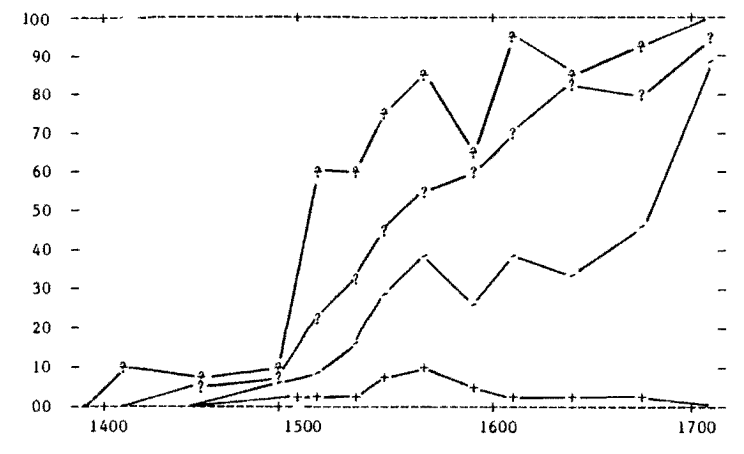
\includegraphics[width=.8\linewidth]{output/images/kroch-graph}
		\caption{Frequency of do-support in different environments: affirmative and negative questions (? and \sout{?}) and affirmative and negative declaratives (+ and ') (Fig. 1 from \citealt{Kroch.1989})}
		\label{fig:kroch-graph}
	\end{figure}

	In summary, quantitative diachronic syntax relies on logistic regression models to provide statistical comparison between various changes. The Constant Rate Effect occurs when a change spread through at least two different syntactic contexts at the same rate. This effect can be identified by the lack of a significant interaction between variables representing the different contexts and the variable representing year of composition. The interpretation of the Constant Rate Effect is that in such cases there is one grammatical change that has reflexes in multiple contexts, which means that quantitative corpus data can reveal information about the structure of the grammatical architecture (namely whether or not two surface constructions share an underlying grammatical derivation).

\section{Recipient Marking}
\subsection{Dative P Allomorphy}
This section shows how data from the history of English supports the allomorphy analysis of dative shift. As discussed in Chapter \ref{ch:active}, dative shift is the modern English phenomenon, where the recipient is unmarked when adjacent to the verb (e.g., ``John gave Mary the ball''), but marked with \textit{to} elsewhere (e.g., ``John gave the ball to Mary''). This can be captured with the pair of vocabulary items in (\ref{ex:eng-ds-vi}). This section shows how this grammar arose in the history of English. In order to support the claim that the absence of recipient marking in sentences like ``John gave Mary the ball'' reflects null allomorphy of the P head, I report a finding of the Constant Rate Effect. In particular, I provide evidence for a uniform To Item across all recipient contexts.  

	\begin{exe}
		\ex Examples:
		\begin{xlist}
			\ex John gave (*to) Mary the book.
			\ex John gave the book *(to) Mary.
		\end{xlist}
		\ex Vocabulary Items:\label{ex:eng-ds-vi}
		\begin{xlist}
			\ex Null Allomorph Item: /$\emptyset$/ $\leftrightarrow$ [dative P] / verb$^{\smallfrown}$\_
			\ex To Item: /tu/ $\leftrightarrow$ [dative P]
		\end{xlist}
	\end{exe}

	In order to study the use of \textit{to} for dative P in previous stages of the language, I extracted all tokens from the Parsed Corpora of Historical English \citep{Kroch.2000,Taylor.2003,Kroch.2004,Taylor.2006,Kroch.2010} containing the following recipient introducing verbs (verbs that also introduce goals, e.g., SEND, were excluded): ALLOT, APPOINT, ASSIGN, AYEVEN, BEHIEGHT, BEQUEATH, BETAKE, DAELAN, FEED, GIVE, GRANT, LEND, OFFER, OWE, PAY, PROFFER, PROMISE, RESTORE, SELL, SELLAN, SERVE, SHOW, VOUCHSAFE, and YIELD. I also extracted information about whether the arguments were full noun phrases or pronouns, the relative order of the recipient and theme (and their order with respect to the verb to rule out cases of topicalisation), and whether or not the recipient was marked with \textit{to} (passive data was also collected, which is discussed in Section \ref{sec:en-pas}).\footnote{See Appendix A for links to the queries used in collecting this data.} While I delay a detailed quantitative examination of the corpus results till the next subsection, Figure \ref{fig:to-use} shows the raw frequency of \textit{to} in various time phrases as well as the predicted frequencies according to the optimal model discussed in the next subsection. In this subsection, I provide a qualitative summary of the different stages of English. Since the availability of cliticisation makes data from theme pronouns more complicated, in these two subsections, I focus on cases with full noun phrase themes (e.g., ``John gave Mary the book''). I return to the case of theme pronouns in Section \ref{sec:act-tp}.

	\begin{figure}[ht!]
		\includegraphics[width=\linewidth]{output/images/to-use}
		\caption{Predicted frequency of \textit{to} with full noun phrase themes according to optimal model with raw means shown as points}
		\label{fig:to-use}
	\end{figure}

	None of the vocabulary items in (\ref{ex:eng-ds-vi}) were inherited from Old English. Old English had synthetic dative case marking, where the dative P head was realised as null (\ref{ex:old-eng-vi}), but its features were copied onto elements of the noun phrase through concord and realised on determiners, adjectives and noun heads as synthetic dative case. A consequence of the concord is that even though dative P was itself not realised phonologically, its features were phonologically realised on elements in the noun phrase. 
	\begin{exe}
		\ex Examples using Both Word Orders:
		\begin{xlist}
			\ex \gll and sealde healfne dael (*to) \TH am gesaeligan \TH earfan\\
			and gave half portion.ACC to the.DAT blessed.DAT needy.DAT\\
			\trans ` and gave a half portion to the blessed needy (coaelive.03,+ALS\_[Martin]:69.6009)'
			\ex \gll Man sceal eac syllan (*to) \TH am seocan men husel\\
			one should also give to the.DAT sick.DAT man.DAT eucharist.ACC\\
			\trans `One should also give the sick man eucharist (coaelhom.03,+AHom\_11:177.1583)'
		\end{xlist}
		\ex Vocabulary Items (6th--11th Centuries):\label{ex:old-eng-vi}
		\begin{xlist}
			\ex Universal Null Item:  /$\emptyset$/ $\leftrightarrow$ [dative P]
		\end{xlist}
	\end{exe}
	
	By the end of the Old English period (11th century), the morphological distinction between accusative and dative case inside the noun phrase was breaking down (i.e., the concord between the P head and elements in the noun phrase was no longer being clearly marked). Case marking on nouns, adjectives and determiners was no longer reliable. Both accusative and dative pronominal forms were still being used, but the forms were no longer consistently associated with dative and accusative case (i.e., old dative case forms would be used where previously accusative case was required and vis-a-versa). Around this time, \textit{to} began to be used for the first time to introduce recipients. In Old English, \textit{to} had previously been restricted to goals and addressees, i.e., the indirect object of verbs of communication \citep{Allen.1999,McFadden.2002,OED.2013}. 
	
	Under the analysis proposed here, language learners do not need to learn the existence of the dative P head, since it is always present in recipient constructions. Language learners do need to learn how the P head is realised. In Old English, the syntactic/semantic content of the P head was realised through concord on elements of the noun phrase. When the concord elements were lost, there was no longer any overt realisation of the recipient theta role. The fact that learners quickly reanalysed the goal marking \textit{to} as the realisation of a recipient P head shows that learners \textbf{proactively} seek realisations for syntactic/semantic content. In other words, a grammar with no overt marking of the recipient theta role is a possible natural language grammar (it was produced by adults in the 11th and 12th centuries), but it is diachronically unstable, because the language learning algorithm is biased towards assigning overt realisations to universally provided syntactic/semantic content, such as the recipient P.

	This reanalysis of goal \textit{to} as a possible recipient marker provides the first change in recipient marking, by introducing the To Item into the list of potential vocabulary items for speakers of English. The new grammar of English after the introduction of the To Item is shown in (\ref{ex:simple-vis-eng}). Since neither of the vocabulary items are more specific than the other, and both realise the same syntactic/semantic features, the grammar is unable to determine which item to use, which is the classic situation of grammar competition. As shown in Chapter \ref{ch:active}, the use of \textit{to} in RT orders (\ref{ex:mideng-rt-to}) cannot be attributed to Heavy NP shift, but must reflect underlying use of \textit{to} in RT orders, which supports the idea that both $\emptyset$ and \textit{to} were unrestricted in distribution). 
	\begin{exe}
		\ex Examples of Both Word Orders (spelling modernized and obsolete words translated in parentheses):
		\begin{xlist}
			\ex I have given \textbf{Purry} a gown (PASTON,I,232.2716)
			\ex They gave \textbf{to the people} this bread (CMWYCSER-M3,248.452)\label{ex:mideng-rt-to}
			\ex Thou givest thine aught (possessions) \textbf{God} (CMVICES1-M1,37.437)
			\ex Lord, in thy will, thou gave virtue \textbf{to my fairness} (CMEARLPS-M2,32.1360)
		\end{xlist}
		\ex Vocabulary Items (11th--14th Centuries):\label{ex:simple-vis-eng}
		\begin{xlist}
			\ex Universal Null Item: /$\emptyset$/ $\leftrightarrow$ [dative P]
			\ex To Item: /tu/ $\leftrightarrow$ [dative P]
		\end{xlist}
	\end{exe}

	The unrestricted distribution of \textit{to} and $\emptyset$ lasted until the 14th century. Throughout this period, \textit{to} use was more frequent in TR (theme--recipient) contexts (e.g., ``John gave the book (to) Mary'') than in RT contexts (e.g., ``John gave Mary the book''). If the recipient use of \textit{to} came from a reanalysis of the goal use of \textit{to}, this would explain the order asymmetry, since goal \textit{to} (as a traditional prepositional object) is base merged as a complement of the main verb and has the end of the verb phrase as its default word order. Our prediction of this explanation is that the TR/RT asymmetry should be insensitive to OV vs. VO word order, since the verb adjacency constraint is a later development that is used to explain the asymmetry by later language learners, rather than the origin of the asymmetry. This prediction is validated in Dutch, which has OV word order, but shows the same TR/RT asymmetry as Middle and Early Modern English.
	
	By the end of the 14th century, \textit{to} has become categorical in the TR order, while it still alternates with $\emptyset$ in the RT order. Once $\emptyset$ has become sufficiently rare in the TR order, some learners will by chance receive input with no examples of $\emptyset$ in TR orders (i.e., *``John gave the book Mary''). If the TR order was the only context recipients occurred in, then the grammar of English could have been reduced to having a single Vocabulary Item (the To Item). However, a Null Vocabulary Item is still necessary in order to account for the availability of $\emptyset$ in RT orders (e.g., ``John gave Mary the book''). In order to interpret the variation between 100\% \textit{to} use in the RT context and 50\% \textit{to} use in the RT context as a \textbf{grammatical} feature, children needed to find a local contextual clue to trigger the allomorphy (see the discussion above for the locality constraints on contextual allomorphy). Because Early Modern English had VO word order, the recipient was frequently linearly adjacent to the verb in RT orders. Thus, the RT order was able to be reanalysed as a grammatical condition of verb adjacency. The subsequent loss of verb raising in English (as part of the rise of do-support) removed the final exceptions to this generalisation (namely adverbial interveners between a finite verb and the recipient, e.g., ``John gave quickly Mary the book"). This adjacency to the verb was interpreted as a contextual cue for the distribution of $\emptyset$. The default realisation of [dative P] became \textit{to} and $\emptyset$ was restricted to a contextually specified allomorph. While this allomorph was actuated in the 14th century, it took until the 18th century for it to go to completion. During this 400 year period, the To Item was an invariable part of the grammar, but the Null Allomorph Item was only variably included in the list of Vocabulary Items. This state of affairs is presented formally in the following example:

	\begin{exe}
		\ex Vocabulary Items (14th--18th Centuries):
		\begin{xlist}
			\ex (Null Allomorph Item: /$\emptyset$/ $\leftrightarrow$ [dative P] / verb$^{\smallfrown}$\_)
			\ex To Item: /tu/ $\leftrightarrow$ [dative P]
		\end{xlist}
	\end{exe}

	The list of Vocabulary Items during the 14th--18th Centuries is identical to that of the modern grammar. The difference between the two grammars is that during the earlier period the Null Allomorph Item was only variably used. In other words, the Null Allomorph Item competed with the absence of a Vocabulary Item. This competition reflects the fact that \textit{to} was still used in the RT order during this time period. By the middle of the 18th century, the use of \textit{to} in RT contexts is the same as in the modern grammar (i.e., only grammatical when derived via Heavy NP Shift). If learners simply adopted the Null Allomorph Item wholesale, the rate of \textit{to} use in RT contexts would have instantly dropped to modern levels. As will be shown in detail in the next subsection, the rate of \textit{to} slowly decreased over the subsequent four centuries to reach modern levels.
	
	The competition of the Null Allomorph Item (122a) with the absence of an item reflects a case of \textbf{specialisation}. In Middle English, $\emptyset$ and \textit{to} were competing for the realisation of the recipient preposition across the board. Specialisation occurred when $\emptyset$ stopped competing with \textit{to} in the TR context, because the rate of \textit{to} use in that context was indistinguishable from 100\%. At that point, the variation between \textit{to} and $\emptyset$ was grammaticalised, by actuating the Null Allomorph Item. However, the primary linguistic data had more use of \textit{to} than would be predicted by the new grammar with the Null Allomorph Item. Therefore, learners needed both the new grammar and the old grammar that \textbf{only} contained the To Item in order to capture the frequency of \textit{to} in the surrounding speech community. Note that the To Item is identical between the two grammars, the only difference is the presence/absence of the Null Allomorphy Item. Thus, the development of specialisation (where the grammar becomes more complex by introducing contextual allomorphy) is driven by the competition between the new allomorph and the absence of that allomorph.

	\cite{Wallenberg.2013} argued that grammar competition inevitably results in one of two possible outcomes: (i) one of the competitors drives out the alternatives or (ii) the grammar specialises the competitors and restricts them to different contexts. The evidence from the rise of \textit{to} in English suggests that this specialisation can be driven by a learning heuristic that disprefers variation. Once probabilistic mechanisms have been introduced into the language machinery, a real question arises if there is any need for anything beyond the probabilistic mechanisms. Any probabilistic system is capable of accounting for categorical data by assigning 100\% (or 0\%) to the relevant forms. The data presented here provides evidence for the existence of a distinction between categorical and probabilistic systems in language use with a learning bias towards categorical analyses of Primary Linguistic Data. In the 14th century, it would have been possible to maintain the 11th--14th century grammar, and simply assign a 100\% probability to the use of the To Item in the TR context and a lower probability in the RT context. However, learners were averse to having surface categorical behaviour be driven by coincidental 100\% probability, instead they interpreted the surface 100\% realisation in TR orders as evidence of categorical behaviour and constructed their grammar accordingly.

	This specialisation was possible because of the following three properties of the grammar and language use in the 14th century. The first, as already described, is the fact that the use of \textit{to} had reached nearly 100\% in the TR context. The second property is the fact that $\emptyset$ still had a substantial presence in the RT context, so it was not possible for learners to simply adopt the To Item across the board. Finally, the third property was the fact that English grammar provided verb adjacency as a context to associate the remaining $\emptyset$ forms in RT context. If English did not provide a salient trigger with the proper grammatical properties (namely consistent adjacency of the recipient preposition to the verb in the RT context), specialisation would have been impossible. This predicts that this type of specialisation should be impossible in OV languages like Dutch, since the verb will not be adjacent to the recipient and thus fail to provide a salient cue for the distribution of the $\emptyset$ form. 

	To properly test this prediction would require looking at a parsed corpus of historical Dutch, which does not exist at this point in time. However, the currently typological evidence is suggestive. Of the Germanic languages that have adopted overt realisation of the dative P head (i.e., Danish, English, Swedish, Norwegian, Dutch and Afrikaans), all of the VO languages have developed the modern English grammar (where overt realisation is obligatory in TR order and the empty set is obligatory in RT order). Dutch and Afrikaans have obligatory overt realisation in the TR context, but optional overt realisation in RT contexts (i.e., they show a similar distribution as in 14th--17th century English without the contextual cue of the verbs). The currently open question is whether the grammar is progressing towards one in which To is obligatory in all contexts, or whether they have adopted some other cue for the distribution of $\emptyset$. The answer to this question awaits the public distribution of a parsed corpus of historical Dutch.

	Returning to VO languages, we find that all of the mainland Scandinavian languages (Norwegian, Swedish and Danish) have the pattern of \textit{to} in TR contexts and no \textit{to} in RT contexts.\footnote{This same pattern is also repeated in many other languages, including with other types of theta roles. In many of these languages, the data is more problematic for my account, since the variation between overt/null preposition coincides with an alternation between overt/null applicative morphemes (see \citet{Baker.1988} for a discussion of the alternation in languages with applicative morphemes). I do not have an explanation for the applicative alternation.} Given that the synchronic explanation for this phenomenon relies on contextual allomorphy, it is non-predicted that the same allomorphy pattern would reoccur in language after language. While the analysis given here does not provide a synchronic explanation for the typological patterns, the \textbf{historical} analysis suggests an explanation. As discussed above, the RT=null/TR=overt pattern found in English was not purely the consequence of accident (e.g., series of independent phonological changes that underly many cases of allomorphy). Instead, the pattern is derived from the origin of the prepositional marker in Prepositional Object Constructions. Thus, as long as languages are deriving their prepositional objects from the same source, it is plausible that the same learning trajectory would repeat in language after language. This is similar to the pattern of common sound changes occurring over and over again producing the same surface patterns (e.g., palatalised consonants before front vowels). While the distribution of null and overt forms in the synchronic grammar is purely accidental, there are strong historical reasons to expect that the same series of accidents would occur in language after language. This claim makes a strong prediction about the historical pattern in other languages that have the RT=null/TR=overt pattern, namely that those languages would show the same rise--fall pattern seen in the history of English.

	\subsection{Quantitative Analysis of the Rise of \textit{to}}
		The previous subsection claimed that the rise in \textit{to} use during the Middle English period reflected the uniform adoption of the To Item, which applied even in RT contexts. A quantitative prediction of this analysis is that a Constant Rate Effect should be found across all contexts in this period. Data was collected from four contexts: (i) TR with recipient noun, (ii) TR with recipient pronoun, (iii) RT with recipient noun, and (iv) RT with recipient pronoun. In order to test the Constant Rate Effect, it is necessary to create a mathematical model for the rate of \textit{to} in these contexts.
	
		For the two TR contexts (with full noun phrase and pronominal recipients), this rise can be modelled with the standard logistic regression models, since they show the typical 0\%--100\% S-shaped curve. The RT contexts require a different model, since \textit{to} rises from the 11th till the 14th century and then decreases in use until the 18th century (as seen in Figure \ref{fig:to-use}). The simple mathematical correlate to the qualitative model discussed above is to use a \textbf{piecewise} function. 
	
		Using a piecewise function, different logistic equations are used depending on whether the reanalysis point in the 14th century has been reached. Up until the reanalysis point in the 14th century, this context will be modelled with a logistic equation with a positive slope (i.e., the frequency of \textit{to} should increase). A Constant Rate Effect would hold between the RT contexts and the TR contexts if the slope of the first half of the RT function is the same as the slope predicted for the TR contexts. After the reanalysis point, a new logistic equation with a negative slope would be used, which would capture the decrease in frequency of \textit{to} from the 14th through the 18th century.

	For the piecewise function, there is one more constraint that is necessary. The frequency predicted by the two equations (before and after the reanalysis point) should be the same at the reanalysis point. This equality is necessary to capture the fact that when the learners do the reanalysis the distribution of the two forms in the newly proposed grammar would be chosen so that they would match the frequencies generated by the pre-reanalysis grammar. This equivalence is captured formally by selecting intercept terms for the second equation that (given a particular slope) generate the correct frequency at the reanalysis point. Therefore, the intercepts in the second function do not need to be estimated, once the reanalysis year has been selected.

	All of the parameters were estimated using Bayesian Inference with RSTAN \citep{stan.2016}. The results of relevance to the Constant Rate Effect are presented in Table \ref{tab:to-mcmc}, where plausible values are defined as being within the 95\% uncertainty interval. As discussed above, Bayesian Inference tests for the Constant Rate Effect by seeing if zero is a plausible value (i.e., if zero is in the uncertainty interval). If zero is \textbf{not} within the uncertainty interval, then zero should not be treated as a plausible value for the interaction and the data provide evidence against the existence of a Constant Rate Effect.

\input{'output/tables/to-mcmc.tex'}

   The results reflect a number of distinct tests for the Constant Rate Hypothesis. In general, the results support two major conclusions. First, the data is consistent with the analysis presented in the previous subsection, where the early rise of \textit{to} is derived from the spread of the To Item through the grammar impacting all ditransitive constructions simultaneously. This conclusion is supported by the CRE findings between RT and TR word orders for the rise of \textit{to}. CH1 Interaction (b) shows that the data is consistent with a Constant Rate Effect in the rise of \textit{to} between sentences like "I gave the books (to) John" and "I gave (to) John the books". CH1 Interaction (d) shows an even stronger example of the Constant Rate Effect for similar sentences with pronouns (e.g., "I gave the books (to) him" and "I gave (to) him the books"). These results bolster the theoretical claims about the nature of the change given in the previous subsection.

   However, the quantitative analysis also reveals that there is a disconnect between the spread of \textit{to} between nouns and pronouns. In the previous subsection, the assumption was that nouns and pronouns behaved identically with respect to the realisation of the dative P head. The CH1 Interaction (a) shows that there was \textbf{not} a Constant Rate Effect finding between sentences like "I gave the book (to) John" and "I gave the book (to) him". The use of \textit{to} with pronouns seems to have been actuated later than its use with nouns, but then spread through the grammar quicker (as can be seen in Figure \ref{fig:to-use} on page \pageref{fig:to-use}). It was also the case that sentences like "I gave (to) him the book" behaved more like "I gave the book (to) him" than to "I gave the book (to) John", with zero on the border of plausible values for the comparison between "I gave (to) him the book" and "I gave the book (to) John" (CH1 Interaction c). Finally, the development of the null form in RT contexts did not show a constant rate effect (CH2 Interaction), with pronouns showing a faster development of the null form. Together, these three pieces of evidence suggest that recipient pronouns and recipient noun phrases reflect different morphological systems.

   Given the difference between nouns and pronouns in both changes, it would have been reasonable for the reanalysis points to be different. The data from the parsed corpora are consistent with recipient nouns and pronouns sharing the same reanalysis point. However, if there is a difference between nouns and pronouns, it is likely that pronouns had a later reanalysis point than nouns (Reanalysis Diff). This is consistent with the analysis presented above, where high rates of \textit{to} use in TR clauses drove the reanalysis in RT clauses. Since the use of \textit{to} went to completion in TR clauses later with pronouns than with full noun phrases, it was predicted that the reanalysis point for pronouns be slightly later than for full noun phrases.

   Such a difference between the morphological realisation of nouns and pronouns is not uncommon cross-linguistically. Indeed, most of the Romance languages have the property where clitic recipient pronouns have a null dative P head, while full noun phrase recipients and non-clitic pronouns have an overt dative P head (in the Romance equivalent of \textit{to}). It may be the case that the difference in English also reflects a difference between clitic and non-clitic pronouns in English. In the next sub-section, I discuss other evidence for the existence of pronoun cliticisation in English and its impact on the morphological realisation of the dative P head.
    
	\subsection{Pronoun Cliticisation}\label{sec:act-tp}
	In this subsection, I present evidence of special behaviour by pronouns, focusing of data where the theme is a pronoun. When the theme is a pronoun, the TR order was essentially categorical (31 examples of RT order over 1000 years out of 712 examples with theme pronouns). Since there was such poor evidence for the frequency of \textit{to} use in these environments, their inclusion muddled any attempts at statistical analysis. Therefore, those cases have been excluded for the analyses discussed below. Instead, I focus on cases where with a theme pronoun and a TR order.

	As discussed in Chapter \ref{ch:active}, theme pronoun cliticisation can produce surface violations of the generalisation that the null allomorph of the dative P head only occurs adjacent to the verb (e.g., ``John gave it Mary''). The theme pronoun does not intervene once it has cliticised, because it is considered morphologically to be a part of the verb. I showed that in some dialects of Northwestern British English, this process still occurred:

	\begin{exe}
		\exr{ex:nw-brit-P} Northwestern British English:
		\begin{xlist}
		\ex[ ]{John [gave=it] [P=$\emptyset$ Mary]}
		\ex[*]{John [gave] [the book] [P=$\emptyset$ Mary]}
	\end{xlist}
	\end{exe}

	The effect of theme pronoun cliticisation can also be seen in the historical data. Figure \ref{fig:brit-tp} shows data from TR word orders with theme pronouns. In both cases, the same rise in \textit{to} as discussed earlier is seen, which just shows the adoption of the To Item. However, instead of levelling out at 100\%, for both recipient noun phrases and recipient pronouns, the logistic regression goes to some point short of completion, which can be explained as reflecting the combination of adopting the Null Allomorphy Item and the rate of theme pronoun cliticisation. For full noun phrase recipients, the rate of \textit{to} use is $\sim$\input{output/tables/fnpr-dtp.tex}, while for pronoun recipients, the rate of \textit{to} use is $\sim$\input{output/tables/pr-dtp.tex}.\footnote{These reflect the average rate of \textit{to} use in these two context between 1425 and 1700.} While theme pronoun cliticisation explains the existence of null marked recipients in these contexts, it does not explain the discrepancy between full noun phrase and pronoun recipients.

	\begin{figure}[ht!]
		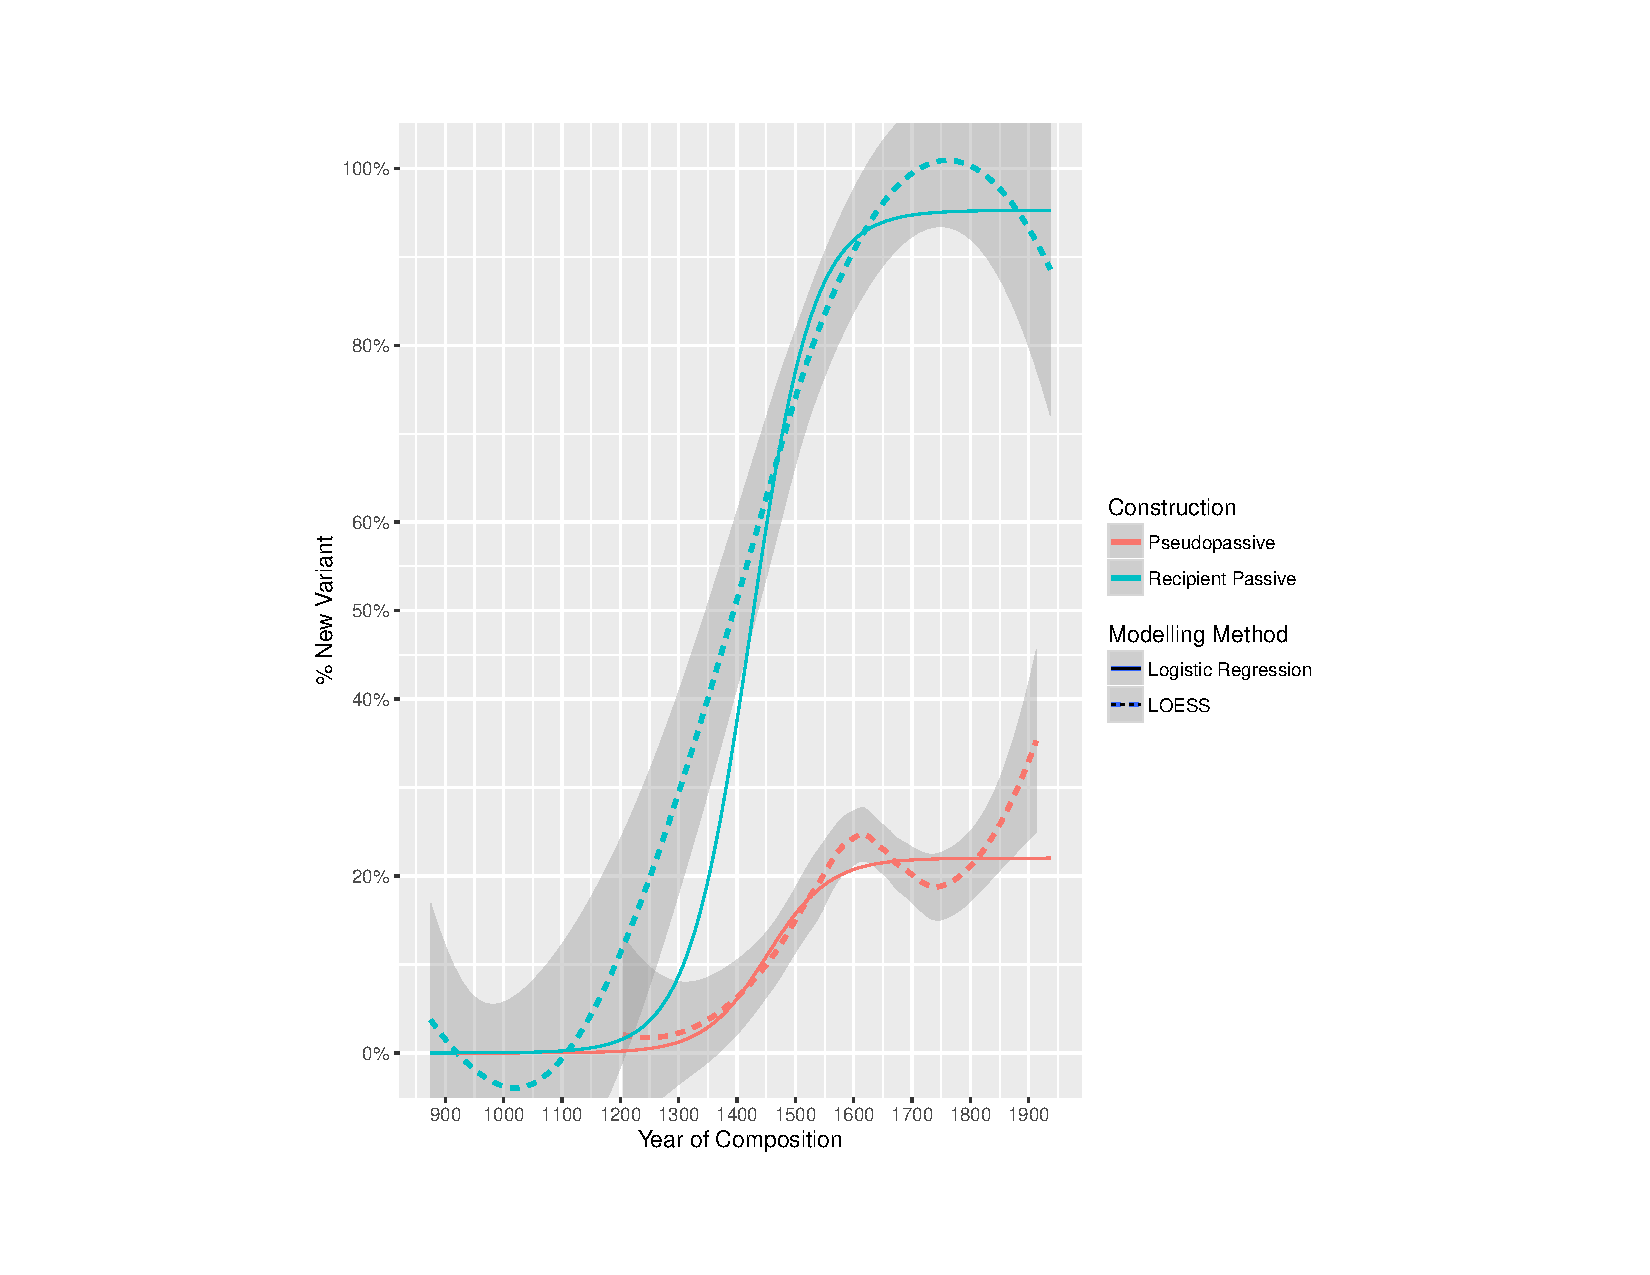
\includegraphics[width=\linewidth]{output/images/brit-tp}
		\caption{LOESS fits for TR data with theme pronouns (points indicate raw frequencies)}
		\label{fig:brit-tp}
	\end{figure}

	In the previous subsection, it was seen that pronoun recipients showed different behaviour from full noun phrase recipients in the adoption of the Null Allomorphy Item. I proposed that this involved a process of recipient pronoun cliticisation, which showed different morphological marking than full noun phrase recipients. The same explanation works for the situation discussed here. Theme cliticisation on its own is fairly rare, as seen by the low rate of null full noun phrase recipients. However, when both the theme and the recipient are pronouns, both pronouns are likely to cliticise, and the null form associated with the recipient pronoun explains the lower rates of \textit{to} use. The propensity for recipient pronouns to be null marked seen both in this subsection and the previous subsection supports the notion that the use of \textit{to} reflects morphological variation that is sensitive to pronominality as is seen in the morphological distinction between clitic and non-clitic pronouns in many Romance varieties.

	As can be seen in Figure \ref{fig:brit-tp}, the difference between pronouns and full noun phrases seems to be shrinking in standard Modern British English (i.e., after 1700). As discussed in chapter \ref{ch:passive}, American English data shows that sentences like ``John gave it Mary'' and ``John gave it him'' were already rare at the beginning of the 19th century in American English and were lost by the middle of the 20th century. While the British data ends in the early 20th century, it seems that the same process was affecting standard British English. It seems both standard British and standard American English lose pronoun cliticisation effects over the 18th, 19th and 20th centuries.

	Additional evidence for cliticisation comes from looking at recipient marking in theme passivisation and how it changes in American English. The relevant change is the loss of direct theme passivisation (e.g., ``The book was given John''), where the theme raises across the recipient to subject position (for more discussion see Chapter \ref{ch:passive}). In English, direct theme passivisation can be identified by the absence of \textit{to} before the recipient. If the theme scrambles to the left of the recipient before raising to subject position, then its lower copy intervenes between the recipient and the verb, preventing the null allomorph from being used (\ref{ex:eng-directtheme}).

\begin{exe}
	\exr{ex:eng-directtheme} English Dialects:
		\begin{xlist}
			\ex[ ]{The book was given P=$\emptyset$ the man \sout{the book}.}
			\ex[*]{The book was given \sout{the book} P=$\emptyset$ the man \sout{the book}.}
		\end{xlist}
\end{exe}
	
	In Chapter \ref{ch:passive}, direct theme passivisation was argued to result from two possible sources: (a) the locality properties of T in looking for a subject to move (i.e., are PPs valid subjects and how many arguments can T consider for subject properties) and (b) recipient pronoun cliticisation. When direct theme passivisation is possible, the recipient is passed over for subject movement either because, as a PP, it is not a valid subject and T can keep looking down the tree to find the theme or because as a clitic it has incorporated into the verbal head. In the new grammar, however, T is no longer allowed to consider multiple arguments. Therefore, the recipient blocks passivisation since T can no longer keep looking and find the theme. The loss of direct theme passivisation can be operationalised as both: (a) the replacement of T with the invisible search property with one with defective intervention and (b) the loss of recipient pronoun cliticisation. The trajectory of this change can be seen in Figure \ref{fig:loss-of-dt-in-amen} on the next page.

	\begin{figure}[ht!]
		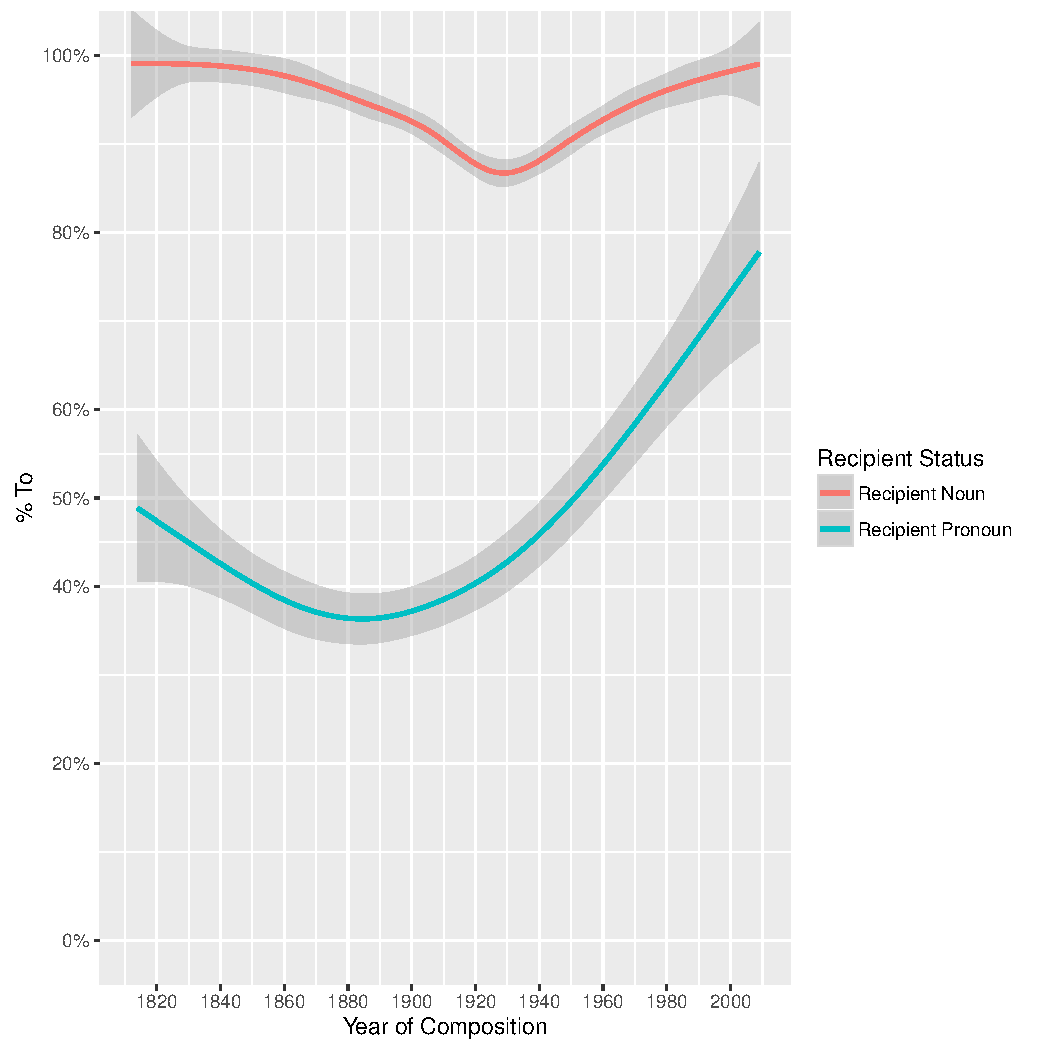
\includegraphics[width=\linewidth]{output/images/directtheme-am}
		\caption{LOESS curves showing the loss of direct theme passivisation with GIVE and OFFER in American English}
		\label{fig:loss-of-dt-in-amen}
	\end{figure}

	The rise/fall pattern seen in the development of direct theme passivisation in American English is discussed further in section \ref{sec:pasrate}. Before turning to that, it is worthwhile to spend a brief moment on the loss of recipient pronoun cliticisation. As can be seen in Figure \ref{fig:loss-of-dt-in-amen}, direct theme passives (absence of \textit{to} with theme passivisation) are much more common with pronoun recipients than full noun phrase recipients, suggesting that pronoun cliticisation was a common operation that could independently derive direct theme passivisation. The higher rates of direct theme passivisation with recipient pronouns can be directly attributed in this case to the fact that there are two independent mechanisms for generating the same surface phenomenon.
	
	In Chapter \ref{ch:passive}, I showed that direct theme passivisation survived in American English after the loss of theme cliticisation (i.e., after sentences like ``I gave it him'' became ungrammatical). While the loss of theme cliticisation and the loss of recipient cliticisation were shown to not be identical, there is a plausible connection between the two. It is plausible that language learners generalise evidence about one type of cliticisation, using the evidence of cliticisation with one type of pronoun as supporting evidence for cliticisation with other types of pronouns. Thus, the loss of theme cliticisation removed a potential source of evidence for the existence of cliticisation in the grammar. It is probably not coincidental that direct theme passivisation begins to decline around the same time that theme cliticisation is lost (i.e., 1940s).
 
	\section{Recipient Passivisation}\label{sec:en-pas}

	The change discussed in this section is the replacement of oblique passives (e.g., 'him was given the book') by nominative recipient passives (e.g., 'he was given the book'). The structure of the section is as follows. First, Old English is discussed and it is argued that the situation is too impoverished to provide clear data, although there is suggestive evidence that Old English had some oblique passives. Secondly, I discuss the change from oblique passives to nominative passives and show that this change co-exists with the rise in pseudopassivisation in English, which supports the notion that nominative recipient passivisation derives from P-incorporation as discussed in Chapter \ref{ch:passive}. 

\subsection{Old English}
	The situation in Old English is quite complex. \cite{Allen.1999} provides evidence that monotransitive datives are able to become oblique subjects in Old English and not topicalised objects. To discuss this distinction, she introduces the term ``fronted dative'', which is agnostic as to whether the fronted element is a topic or a subject. Contrary to her claims about monotransitive datives, she argues that there are no oblique subjects in ditransitive passives, only topicalised objects. This claim is made on the basis of Coordinate Subject Deletion facts. In Old English (as in Modern English), arguments are generally obligatory (i.e., neither subject nor object drop is generally licensed). However, when two sentences are coordinated and share the same subject, the subject does not need to be expressed in the second sentence (\ref{ex:OECSD}). In a corpus investigation, none of the fronted datives in ditransitive passives triggered Coordinate Subject Deletion, while a number of fronted nominatives did (see Table \ref{tab:AllenOECSD}). 

	\begin{table}[t]
		\begin{tabular}{cccc}
			Nominative Coreferential & & Deletion & No Deletion \\
			& Order NOM DAT & 11 & 4 \\
			& Order DAT NOM & 4 & 3 \\
			& Total & 15 & 7 \\
			\hline
			Dative Coreferential & & Deletion & No Deletion \\
			& Order NOM DAT & 0 & 27 \\
			& Order DAT NOM & 0 & 11 \\
			& Total & 0 & 38 \\
		\end{tabular}
		\caption{Allen's counts of Coordinate Subject Deletion with ditransitive passive in OE prose (Table 2-6, \citealt{Allen.1999})}
		\label{tab:AllenOECSD}
	\end{table}

	\begin{exe}
		\ex \label{ex:OECSD} Old English:
		\gll and him comon \textbf{englas} to, and him ðenodon\\
		and him.DAT came \textbf{angels.NOM} to, and him.DAT served\\
		\trans ` and to him angels came and him (they) served \citep[ex. 34]{Allen.1999}.''
	\end{exe}

	The main problem with this conclusion is that there were only a small number of Old English coordinated examples, such that the lack of deletion for datives could be accidental. The problem of whether fronted oblique elements are subjects is not unique to Old English. The same uncertainty hold with respect to Old Norse (see for example \citealt{Kristoffersen.1991,Kristoffersen.1994} and \citealt{Bardal.2001b}). Unfortunately, many of the examples that clearly show that oblique elements are subjects rely on negative data, which is unavailable for earlier states of the language. Because of this problem, I focus instead on data starting with Middle English, where I make the assumption that oblique fronted elements are subjects, since Middle English has developed an obligatorily filled subject position and lost any traces of V2 (or V2-like effects), meaning that the element immediately before the finite verb is the subject.

	\subsection{Rise of Nominative Recipient Passivisation}\label{sec:eng-to-pass}

	As discussed in the previous subsection, I am assuming that Middle English has oblique subjects in cases of fronted recipients. However, since synthetic case marking had been lost (for full noun phrases) by Early Middle English and since the To Grammar (see the previous section) was not yet universal, even with these assumptions, it is difficult to determine whether a fronted recipient was nominative or dative. \cite{Allen.1999}, after carefully examining the extant Middle English corpus, identifies that the first unambiguous case of a nominative recipient subject in the passive of a ditransitive occurs in 1375. This reflects a change in the grammar of English, in so far as previously nominative recipient subjects were ungrammatical and now they are grammatical.

	There are potentially three distinct types of recipient passive. Example (\ref{ex:obliq-rec-eng}) shows an example of oblique passive without \textit{to}. Even though the recipient itself (``the king Gurthym'') is ambiguous between an oblique and nominative structure, the fact that the verb (``were'') agrees in number with the theme (``the provinces'') shows that the theme received nominative case and the recipient subject must be oblique. These kinds of examples are quite rare. Most examples of recipient subjects without \textit{to} are coded as nominative subjects (\ref{ex:nom-rec-eng}), even though their form does not distinguish between an oblique and a nominative analysis. Clear examples of oblique recipient passives can be seen in (\ref{ex:obliq-to-rec-eng}). As discussed in the previous section, the realisation of dative P as \textit{to} became obligatory for non-adjacent constructions by about 1400. At that point, the distinction between \textit{to}-marked (\ref{ex:obliq-to-rec-eng}) and bare recipients (\ref{ex:nom-rec-eng}) becomes an unambiguous indicator of the case of the recipient (namely dative and nominative respectively).

	\begin{exe}
		\ex Middle English \citep{Kroch.2000} and Early Modern English \citep{Kroch.2004}
		\begin{xlist}
			\ex\label{ex:obliq-rec-eng} the king Gurthym, that we clepteth Gurmundus, were i-yeve the provinces of Est Anglia and Northumbria (CMPOLYCH-M3,VI,377.2770)
			\ex\label{ex:nom-rec-eng} for the prioress is given a matter to proud in the beginning of her ordinance (CMBENRULE-M3,43.1346)
			\ex\label{ex:obliq-to-rec-eng} to thy holy name be given laude and praise (STOW-E2-P2,581.96)
		\end{xlist}
	\end{exe}

	Under the analysis described in Chapter \ref{ch:passive}, the nature of this grammar change reflects the availability of P-incorporation. Without P-incorporation, the only possible form of recipient passivisation is to have oblique subjects. Given that P-incorporation also generates pseudopassives, the simple prediction would be that pseudopassives would enter the language at the same time as nominative recipient passives. \cite{Sigursson.2014} showed that pseudopassivisation comes into the language in the beginning of the Middle English period. Indeed, as seen in Figure \ref{fig:recpas-pseudo}, pseudopassivisation and nominative recipient passivisation increase in use from about 1200 until 1650, when they both level off.\footnote{The pseudopassive data here is taken from a hand corrected dataset produced by Sigursson from the Parsed Corpora of Historical English. Using automatic queries, roughly the same number of pseudopassive examples are found, but the number of corresponding actives are much higher. This discrepancy probably derives from a failure to identify a number of criteria that would prevent a possible active from being a potential pseudopassiviser. Since Sigursson curated his dataset for the study of pseudopassivisation, it provides a more reliable dataset and therefore his values are reported here.}

	\begin{figure}[ht!]
		\includegraphics[width=\linewidth]{output/images/recpas-old-pseudo}
		\caption{Logistic regression curves and LOESS curves showing rates of nominative recipient passivisation and pseudopassivisation in English}
		\label{fig:recpas-pseudo}
	\end{figure}

	Neither pseudopassivisation nor nominative recipient passivisation go to 100\%. For pseudopassivisation, this is expected. If the pseudopassivisation rate was 100\% that would mean that there were no active sentences with PP objects, which is highly improbable. For nominative recipient passivisation, it is less clear why the process should not go to completion, since this is the probability of having a nominative subject given that recipient passivisation has occurred, which could reasonably occur 100\% of the time. However, locative inversion remains possible to the present day (\ref{ex:locinv}). There is debate in the literature about the proper analysis of locative inversion, but it seems likely that locative inversion is actually a type of topicalisation and not subject raising \citep{Bresnan.1994}. Ideally, locative inversion should be excluded from our cases, but this cannot be done, since cases of locative inversion are surface identical with the cases of oblique passivisation with \textit{to}.

	\begin{exe}
		\ex Modern English: To the guests were given goblets of gold and silver (\citealt{Bruening.2010}, Ex 26a)\label{ex:locinv}
	\end{exe}

	To summarise, the change from oblique passivisation to nominative passivisation suffers from two surface complications. In the early period, some cases of oblique recipient passivisation have bare recipients, since realisation of dative P as \textit{to} was not yet obligatory. Also, throughout the change, some cases of fronted recipients with \textit{to} represent cases of locative inversion, which properly should not be included, but cannot be distinguished from genuine cases of oblique recipient passivisation. In spite of these complications, it is possible to do quantitative research on the trajectory of the change.

	This change would seem to be a good case to look for a Constant Rate Effect (see Section \ref{sec:log-reg}), namely between the rise of pseudopassivisation and the replacement of oblique recipient passives by nominative recipient passives, since both are proposed to reflect the underlying adoption of P-incorporation into the grammar. However, there are two problems that impede investigation of a constant rate effect. There is a great deal of uncertainty about the rise of nominative recipient passivisation, because there are few cases of recipient passivisation overall (see the next subsection for a discussion of why there is little data). Thus, even if a Constant Rate Effect is found (i.e., there was no significant interaction between year and pseudopassive vs nominative recipient passive), this can be attributed to the lack of data concerning recipient passives. Secondly, the fact that the changes do not go to 100\% means that standard techniques for fitting the logistic regressions cannot be used.

	In order to resolve the second problem (fitting models to data that does not go to 100\%), scaled versions of logistic regression can be used, where the output of the formula for each year is scaled by multiplying the predicted output by a scaling constant reflecting the final rate of usage. For example, assume that the change from oblique recipient passives to nominative recipient passives stabilises at 90\% instead of 100\%. The rate of 90\% is calculated by averaging the rate of all years after the change seems to have stabilised (in this case after 1700). Instead of using the direct output of logistic regression to predict the probability of using a nominative recipient passive in any year, the output of the logistic model is first multiplied by 90\%. The consequence of this process is that at the end of the change the predicted probability is 90\% instead of 100\%. The optimal values for the logistic regression parameters can still be estimated from the data, so a Constant Rate Effect can still be tested for. 

	In this case, a Constant Rate Effect was found. Table \ref{tab:pas-change-tab} shows that zero is a plausible value for the Year:Type interaction. In fact, the effect here is even stronger than the Constant Rate Effect, since the data is compatible with there being no difference at all between the two conditions. Since the data from recipient passives is tentative, the result is only suggestive, but it is most consistent with the notion that the rise of nominative recipient passivisation and pseudopassivisation are derived from the same underlying change, namely the adoption of P-incorporation.

\input{output/tables/recpas-old-mcmc.tex}

	In summary, the rise of nominative recipient passives in English provides tentative additional evidence for the P-incorporation analysis. Nominative recipient passivisation and pseudopassivisation enter the language in the same way, providing another example of the Constant Rate Effect. Since P-incorporation is a standard analysis of pseudopassivisation, the Constant Rate Effect finding supports the notion that nominative recipient passivisation is also derived via P-incorporation when the operation entered the language during the Middle English period. One caveat about the Constant Rate Effect finding was that it was based on only a small amount of data from recipient passives. The next subsection discusses why there are so few recipient passive examples.

	\section{Passivisation and Underlying Word Order}\label{sec:pasrate}

	This subsection discusses a change in American English that supports the analysis of direct theme passivisation as being derived from an underlying RT word order. In particular, before the loss of direct theme passivisation in 20th century American English (as discussed above), recipient passivisation and direct theme passivisation pattern together. In Early Modern and Modern British English, they both show depressed rates, which both increase in American English. While the proper account of the depressed passivisation rate and its subsequent increase are unknown, the fact that recipient passives and direct theme passives pattern together supports the notion that they share some property in common. Under the analyses proposed here, the shared property is passivisation from the RT word order.

	As discussed in the preceding subsection, the grammar of recipient passivisation changed during the Early Modern British period from oblique recipient subjects to nominative recipient subjects. However, during that time, the over all rate of recipient passivisation (as either oblique or nominative) remained constant at about 1\% (as can be seen in Figure \ref{fig:brit-pas} on the next page), which reflects the percentage of passive sentences with RT word order out of all sentences with RT word order. This rate of 1\% is substantially lower than the rate of monotransitive passivisation and the rate of passivisation with TR word order (as shown in Figure \ref{fig:brit-pas}). Table \ref{tab:model-comp-pasrate} on the next page shows that there is a difference in passivisation rates between RT and TR word orders (i.e., 0 is not a plausible value for the difference).
	\input{'output/tables/pas-mcmc.tex'}

	\begin{figure}[ht!]
		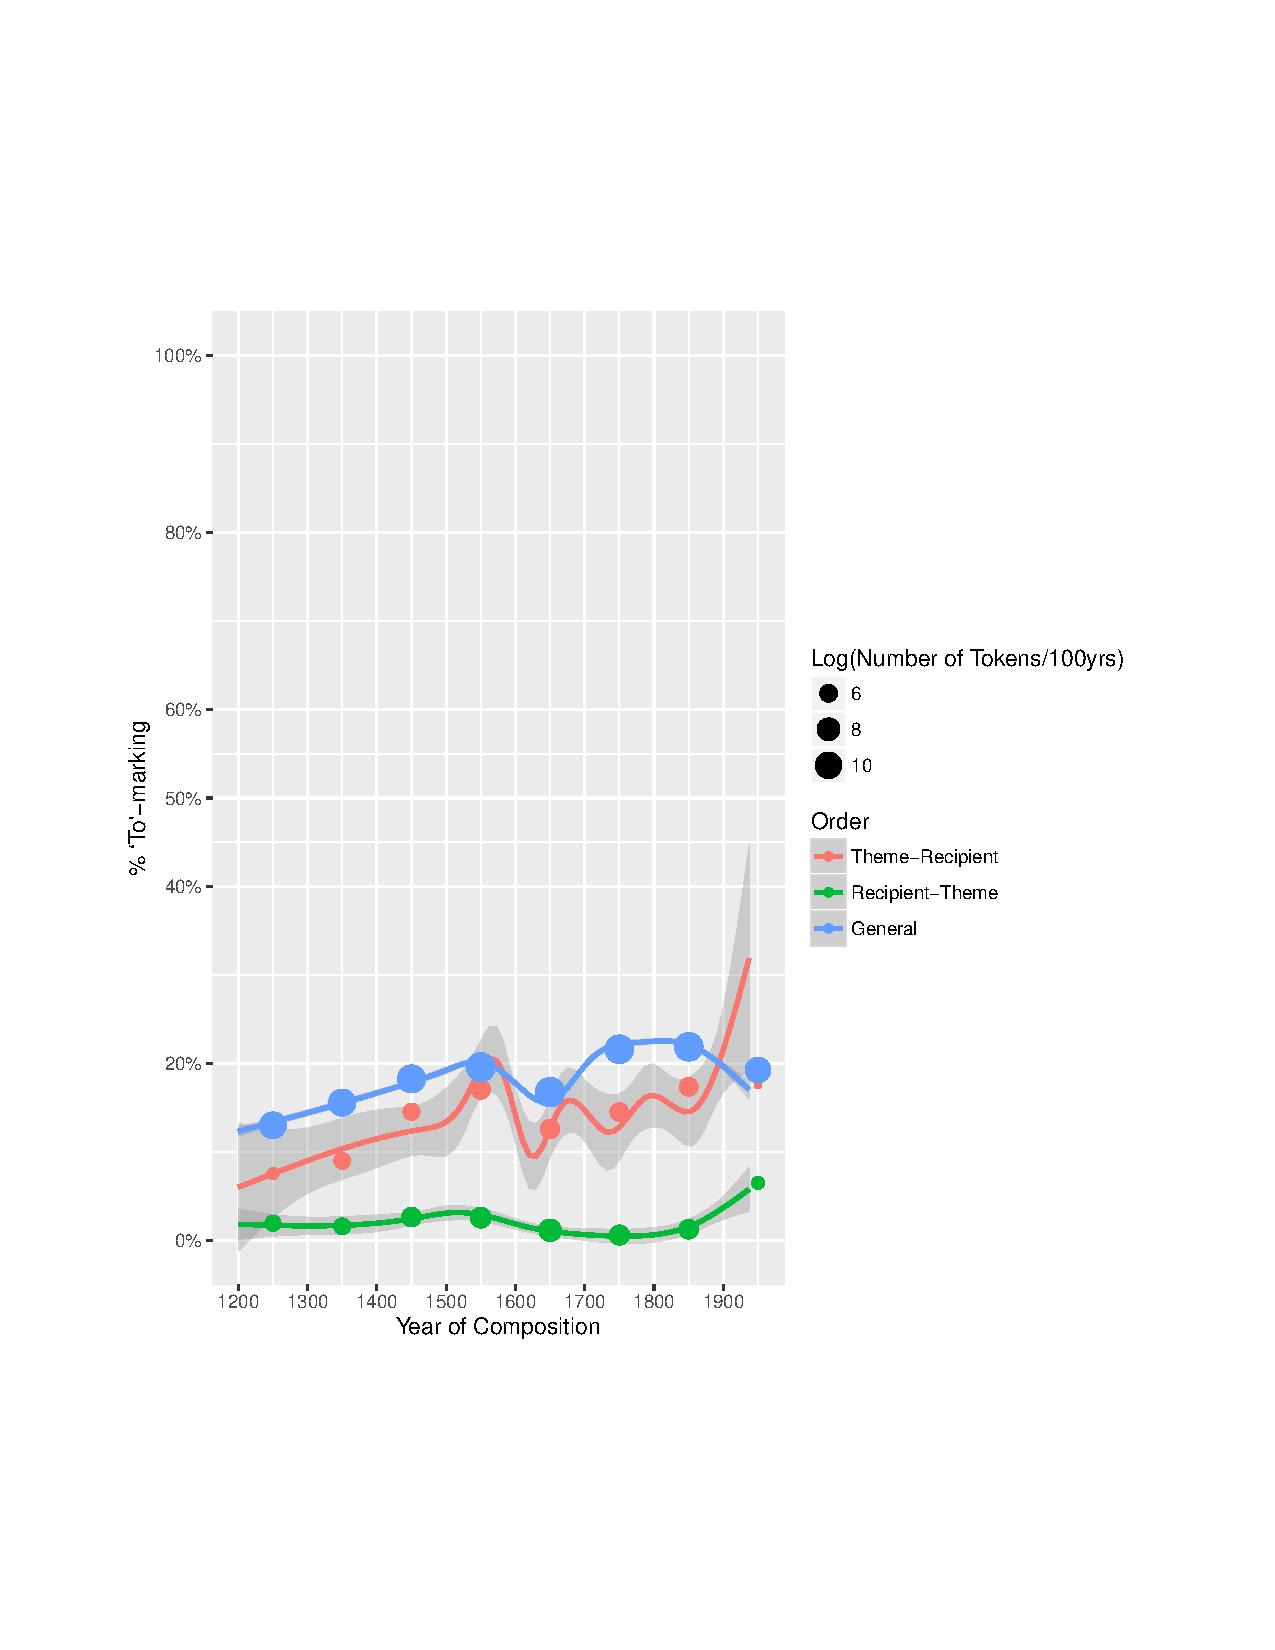
\includegraphics[width=\linewidth]{output/images/brit-pas}
		\caption{LOESS fits for rates of passivisation in TR, recipient theme and general clauses}
		\label{fig:brit-pas}
	\end{figure}

	At the same time, as shown in Figure \ref{fig:brit-tp} on page \pageref{fig:brit-tp}, the rate of direct theme passivisation (i.e., lack of \textit{to} marking on the recipient in a theme passive) with full noun phrase recipients was also low. In both cases, recipient passivisation and direct theme passivisation occur often enough that they are unlikely to be the product of errors and thus should be taken as grammatical, but seem to be seldomly used. The fact that both of these constructions show a marginal status in the British English data is not a particularly strong argument in favour of them sharing an underlying analysis. However, in American English, the marginal status of these constructions goes away at the same time. Figure \ref{fig:am-change-pass} shows the rate of recipient passivisation and direct theme passivisation together in American English with full noun phrase recipients. Throughout the 19th century (i.e., before the loss of direct theme passivisation), the rate of direct theme passivisation and recipient passivisation rise in tandem. The parallel nature of this change can be captured by assuming that whatever the formal properties of the change are, they target passivisation from RT underlying word orders.

	\begin{figure}[ht!]
		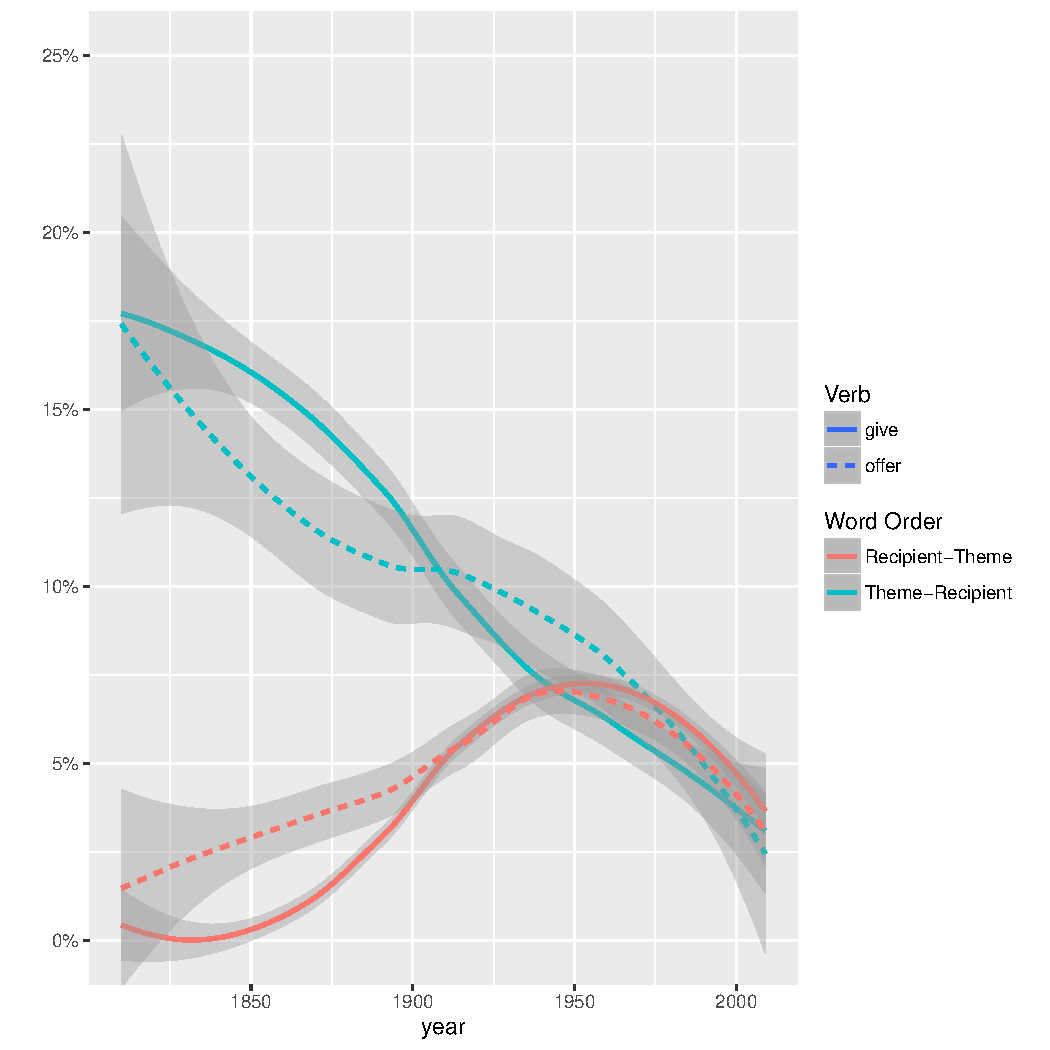
\includegraphics[width=\linewidth]{output/images/am-change-pass}
		\caption{Ditransitive passivisation for GIVE and OFFER from COHA and overall passivisation rate}
		\label{fig:am-change-pass}
	\end{figure}

	I do not have a clear explanation of what formal property changed to produce the change in usage rates in American English. Whatever that formal property is, it specifically targeted the passivisation from underlyingly RT word orders. Throughout Middle and Early Modern English passivisation from underlyingly RT word orders seems marginal in the corpus data (i.e., the usage rates are very low). In 19th century American English, the rate of passivisation in all constructions that are proposed to derive from underlyingly RT word orders in this dissertation increase in usage at the same time. The analysis proposed here (that direct theme passivisation comes from an underlyingly RT word order) is supported by the fact that the two constructions share a shared property under this analysis and the two constructions show parallel development in usage.


\section{Conclusions}
	In this chapter, I showed examples of using quantitative studies in syntactic change to inform linguistic research. This was embedded in a discussion of the nature of linguistic architecture and the relevance of different types of linguistic evidence. Examples were brought to show that quantitative use data can be informative about grammar, but is essential in studying systematic non-grammatical aspects of language.
	
	Looking at the development of recipient marking in English (i.e., the innovation of \textit{to} as the marker of recipients) provided an example of how even complex changes involving the interaction of two distinct changes can be broken apart using relatively simple statistical processes. By breaking apart interacting changes, it is possible to use quantitative measures (such as the Constant Rate Effect) to study the grammatical architecture underlying each change. The quantitative data demonstrated a difference between full noun phrase recipients and pronoun recipients. Within each class, a Constant Rate Effect was found between TR and RT clauses, which supported the uniform analysis of \textit{to} given in this dissertation. However, different slopes were detected between clauses with pronominal recipients and full noun phrase recipients. On the basis of this evidence, I provided an analysis in which pronouns and full noun phrases have different realisations for the recipient P head. While morphological differences between nouns and pronouns are not surprising, given the already known differences between nouns and pronouns in English morphology, this particular difference could not have been discovered without looking at quantitative data.
	
	Looking at recipient passivisation, another case of a clear grammatical change was identified. In particular, both nominative recipient passivisation and pseudopassivisation increase in use during the same time period (Middle and Early Modern English). In this case, there was insufficient data to get strong quantitative results, but the data was consistent with the notion that both nominative recipient passivisation and pseudopassivisation are driven by the same mechanism under this analysis.

	Both of the case studies above show how diachronic syntactic studies can provide independent evidence to support claims made on the basis of synchronic data. In the previous two chapters, I posited two grammatical theories on the basis of synchronic and comparative data: (i) the allomorphy account of dative shift and (ii) the P-incorporation account of nominative recipient passivisation. These grammatical theories made \textit{testable} predictions about diachronic change, in particular predicting Constant Rate Effects. The use of parsed historical corpora provide quantitative data that allows these predictions to be tested. Since the historical data is of a completely different type from the synchronic data (production instead of comprehension; usage rates instead of acceptability judgements), the fact that the synchronic theories predict the diachronic results provides strong independent support to the plausibility of the underlying theories.

	Finally, the rates of recipient passivisation and direct theme passivisation changed together in American English. While there is not clear formal explanation for the change in usage rates, the fact that the use of these two constructions changed in parallel suggests that they share some underlying property (i.e., the property that the change is targeting). I argued that the shared property was passivisation from an underlying RT word order, and used the American English change as another piece of evidence for the analysis of direct theme passivisation as movement of the theme to subject position from an underlying RT word order.

	All of the cases discussed in this chapter shared the property that evidence for particular grammatical analyses was derived from data about the rate at which various grammatical options were used in particular corpora. The underlying logic behind all of these arguments is that concomitant changes in usage reflect a change targeting a particular linguistic property. When two constructions change in parallel, that provides evidence that some change is targeting something shared between the two constructions. By building up a set of constructions that must share \textbf{some} property, it constrains the grammatical analyses to posit some shared property between the different constructions.

%\bibliography{diss}
